\documentclass[10pt]{article}

% File icdp2009.sty
% Preamble that you have to include to use the template  

% July 24, 2009
% Contact: simonnet@ecole.ensicaen.fr


\usepackage[a4paper,textwidth=18cm,textheight=24cm,top=2.85cm, bottom=2.85cm, left=1.5cm, right=1.5cm]{geometry}

\usepackage{../template/icdp2009}

% left justified caption
\makeatletter
\long\def\@makecaption#1#2{%
\vskip\abovecaptionskip
\sbox\@tempboxa{#1. #2}%
\ifdim \wd\@tempboxa >\hsize
#1. #2\par
\else
\global \@minipagefalse
\hb@xt@\hsize{\box\@tempboxa\hfil}%
\fi
\vskip\belowcaptionskip}
\makeatother




%other package

% vectorial font
\usepackage{lmodern}

\usepackage{graphicx}
\usepackage{times}
\usepackage{booktabs}
\usepackage{siunitx}
\usepackage{adjustbox}
\usepackage{multirow}


\begin{document}
\noindent

% This should produce references in the order they appear
\bibliographystyle{ieeetr}

\title{Optical Waveguides: Theory and Implementation}

\authorname{Anirudh Prakash, Grace Liu, Surya Chandramouleeswaran}
\authoraddr{\textbf{\emph{A special thanks to Professor Maysam Chamanzar}}}



\maketitle


\abstract
Replace this with a succint summary of our work. Aim for 100 words  

\section{Introductory Concepts and Motivations}

As the 20th century saw a massive growth in electronic and nanofabrication, there was an increased motive to deliver an analog of an electronic integrated circuit using photons as a unit of data as opposed to electrons in classical analog circuits. This particular application is called integrated photonics, and photonic integrated circuits (PIC) are the devices that utilize this type of technology to include functioning optical components that can process or generate light. We are interested in this topic since optical communication plays a huge role in peoples’ everyday lives, whether from personal cellphones to projects on bigger scales. The major advance in this light-based silicon photonic chip comes with many benefits, including its higher speed, greater area efficiency, lower power dissipation, and increased signal strength. While these advantages seem endless, there are still quite a feel challenges during the process of designing and manufacturing these types of devices. For instance, how can high precision be achieved while optimizing material performance without considering electronic properties? This leads into our main concern of how light can be controlled without the notion of the change in potential energy of electrons since this cannot easily be accomplished without any force.


\begin{figure}[h]
    \centering
    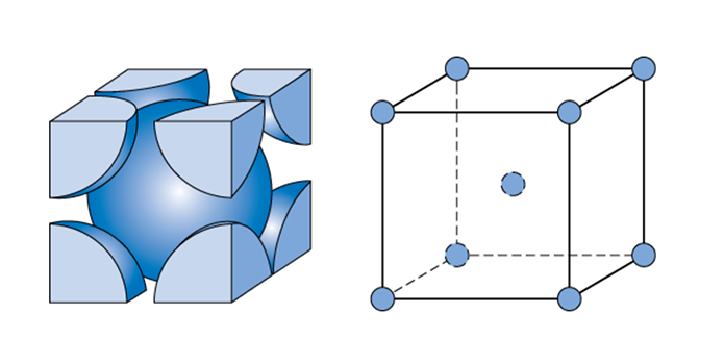
\includegraphics[width=8.5cm]{fig1.eps}
    \caption{\label{tab1}BCC Unit Cell structure, with an atom at the center of the "body" of the cell. Adapted from \cite{ref01}.} 
    \end{figure}

\section{Historical Contextualizations}

Integrated circuits can be dated back to the 1950s when Jack Kilby built the first one at Texas Instruments in 1958. The term “photonics,” or the science involving applications of light, was popularized to replace electronic technologies after the invention of the diode laser. While glass fiber technologies have been around since the 19th century, advancements in photonics allowed for the development of low-loss optical fibers. These are optimal to use in long distance communication since they can minimize signal loss of light traveling through the fiber. The high purity of the silica glass it is typically made out of also helps increase light absorption. The term “integrated photonics” was first coined in the 1980s by a group of researchers at Delft University of Technology, with goals of integrating miniaturization and enhanced functionality onto singular chips. Meint Smith from this group is accredited with inventing the Arrayed Waveguide Grating (AWG) that is applied a lot in modern digital connections to improve signal integrity. Approaching the first decade of the 20th century, the Telecommunications Revolution encouraged various communication methods enabled by advancements in optical waveguides, serving as a transmission medium between communication systems. Now we are equipped with mobile phones, wireless communication, digitalized services, and various other transmission technologies. Transitioning into nowadays, waveguides and photonics can be applied to sensors, biomedical devices, and quantum computing. While photonic sensors offer high sensitivity and immunity to electromagnetic interference, quantum-enhanced sensors use quantum states of light to improve overall performance.

\begin{figure}[h]
    \centering
    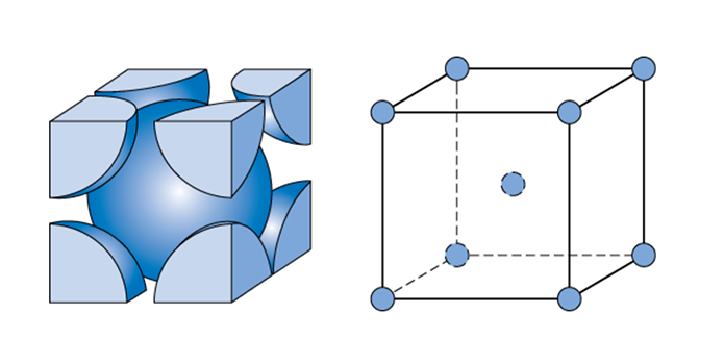
\includegraphics[width=8.5cm]{fig1.eps}
    \caption{\label{tab1}BCC Unit Cell structure, with an atom at the center of the "body" of the cell. Adapted from \cite{ref01}.} 
    \end{figure}

\section{Propagation of Light}

Here we discuss EM mechanisms. Start fundamental and work our way up 


\begin{figure}[h]
    \centering
    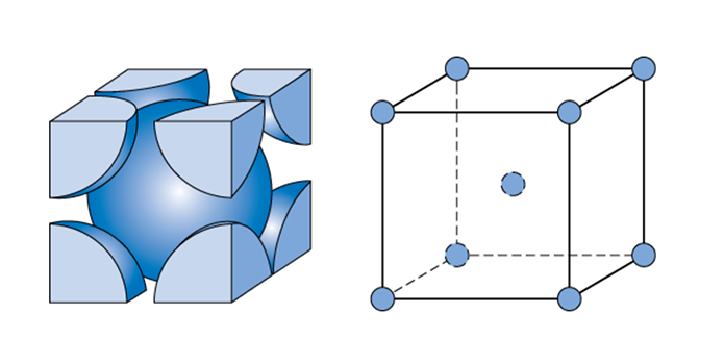
\includegraphics[width=8.5cm]{fig1.eps}
    \caption{\label{tab1}BCC Unit Cell structure, with an atom at the center of the "body" of the cell. Adapted from \cite{ref01}.} 
    \end{figure}

\section{Electromagnetic Mechanisms}

More speciffc here, add TIR and add diagrams and math

\begin{figure}[h]
    \centering
    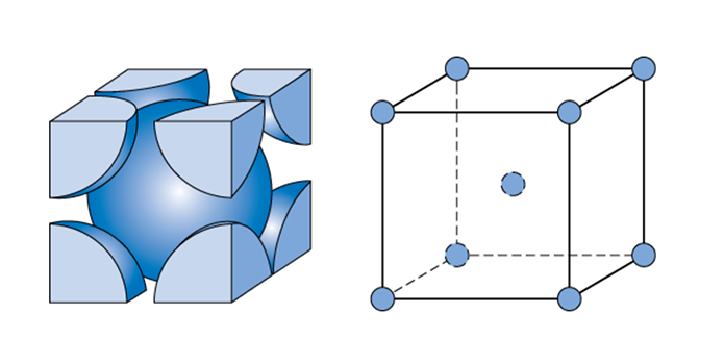
\includegraphics[width=8.5cm]{fig1.eps}
    \caption{\label{tab1}BCC Unit Cell structure, with an atom at the center of the "body" of the cell. Adapted from \cite{ref01}.} 
    \end{figure}

\section{System Integration}

Transitions into some more implmentation details that bleeds into state of art discussion 


\begin{figure}[h]
    \centering
    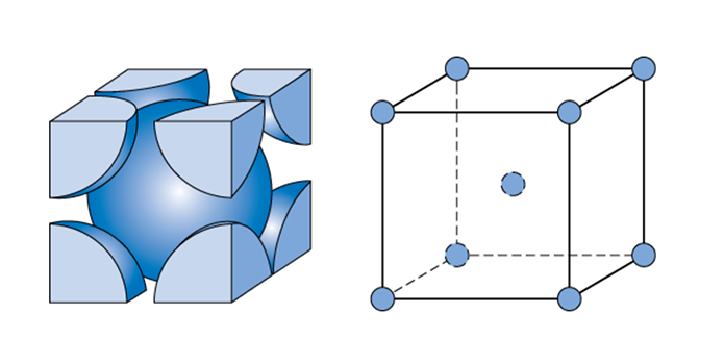
\includegraphics[width=8.5cm]{fig1.eps}
    \caption{\label{tab1}BCC Unit Cell structure, with an atom at the center of the "body" of the cell. Adapted from \cite{ref01}.} 
    \end{figure}

\textbf{Anirudh}: you can decide how you want to organize this 

\section{Evaluation of the State of the Art}

PIC discussion, materials perspective, etc.

The field of integrated photonics is still rapidly evolving, and many advancements have contributed to its growth in the market that is estimated to reach approximately \$29.1 billion by 2026. Optical signals are currently widespread in fiber optic cable usages for long distance communication purposes, permitting higher bandwidths than normal cables would be able to due to the fiber’s inherent material. The phenomenon of total internal reflection enables the fibers to act as an optical waveguide for electromagnetic waves. While optical signals are mainly purposed in telecommunications, other industries like the medical and defense fields also take advantage of such benefits. Beyond telecommunication innovations, photonic integrated circuits are also commercialized in small volumes. By using light instead of electricity, many limitations can be resolved to increase the speed of data transmission. To illustrate this idea, photonics are emerging as a potential innovator for 5G networks to help mitigate high traffic and data rates as opposed to using traditional communication technologies. While photonics present practical solutions, some challenges still remain. Though silicon is one of the most widely used materials to build these circuits, it is not ideal due to its indirect band gap that inhibits its abilities to bond with light emitting devices. Designing these complex devices requires a vast amount of considerations, and there still exists many limitations in their design tools. The level of accuracy is hindered by numerous optical properties that need to be taken account of along with the lack of a standardization. Lastly, there exists the notion of the lack of control over light without the presence of force.



\section{Concluding Thoughts and Ideas for the Future}

self explanatory 




\section{Acknowledgements}

bibliography is very important (references section needs to be modified in example.bib)
\bibliography{IEEEabrv,icdp2009}


\end{document}














